\section{Causal Analysis}
\section{Intro}
\begin{frame}[noframenumbering]{Plan For This Presentation}
  \begin{figure}[h!]
  \centering
    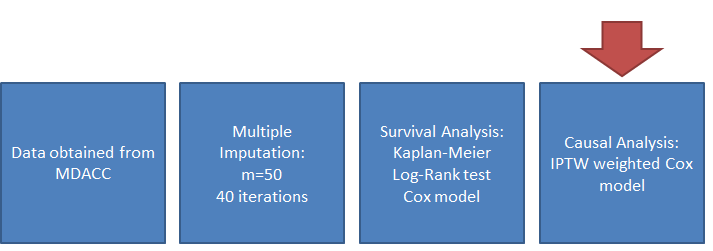
\includegraphics[width=0.9\textwidth]{ps_flow}
\label{fig:ps_flow}
\end{figure} 
\end{frame}

%might want to change this example
\begin{frame}{Causal Analysis}
The treatments were not given in an RCT
 \begin{itemize}
  \item Want to say ``The treatment leads to better survival''
  \begin{itemize}
   \item But need an RCT to say this
   \begin{itemize}
    \item Randomization minimizes differences between groups at baseline
    \item Differences in outcomes are due to treatment
   \end{itemize}
  \end{itemize}
  
   \item We only have observational data
   \begin{itemize}
   \item Differences could be attributed to the drug or confounding factor, e.g.
   
   \begin{itemize}
    \item Healthier patients can tolerate chemo better
    \item Different cancer manifestations lead to different plans\\~\\
   \end{itemize}

   \end{itemize}


 \end{itemize}
 Idea: Try to balance the covariates to reduce the effects of confounding
so the two groups seem identical at baseline
\end{frame}


\begin{frame}{Counterfactuals}
\begin{itemize}
 \item Suppose that for patient $i$, there are two potential outcomes
 \begin{itemize}
  \item $Y_i(0)$ - The outcome if they had taken the control, $T=0$
  \item $Y_i(1)$ - The outcome if they had taken the treatment, $T=1$
 \end{itemize}
 \item The observed value for subject i: $Y_i=Y_i(1)T+Y_i(0)(1-T)$
  \item \textit{The fundamental problem of causal inference}
  \end{itemize}
     \begin{figure}[h!]
  \centering
    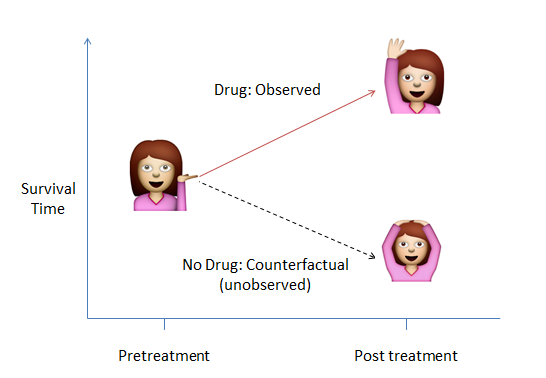
\includegraphics[width=0.5\textwidth]{counterfactual3.png}
    \caption{Example of a counterfactual}
\label{fig:counterfactual}
\end{figure}
\end{frame}



\begin{comment}
 
  
\begin{frame}{Fundamental Problem of Causal Inference}

\begin{itemize}
 \item Obviously we only observe one. \textit{The fundamental problem of causal inference}
\item If we could observe both, then we could observe the causal effects for each person
\end{itemize}
\end{frame}

\end{comment}


\begin{frame}{Rubin's Causal Model: Assumptions}
\begin{itemize}
\item Stable Unit Treatment Value Assumption (SUTVA): Treatment status of another subject does 
not affect outcome of other units. 
%Single version of each treatment
\item Ignorability/No Unmeasured Confounders: $(Y(0),Y(1))\perp T|X$ ,\cite{Rosenbaum1983}
\end{itemize}
\note{No association between outcome and treatment assignment
The ignorability assumption simply means that the choice to assign to the control group
or the treatment group can be assumed to be effectively random when conditioned on observable 
characteristics of the study objects....
knowing whether or not someone is assigned (or chooses) 
treatment contains no information about his what-if outcomes in both treated and untreated states
}
\end{frame}




\begin{frame}{Estimands of Interest}
 \begin{itemize}
 \item Individual Treatment Effect: $Y_i(1)-Y_i(0)$
 \item Average Treatment Effect (ATE): $E[Y(1)-Y(0)]$. The effect of moving entire population
 from treated to untreated
 \item Average treatment effect for the treated (ATT): $E[Y(1)-Y(0)|T=1]$. The average treatment
 effect for those actually treated
 \item Note:  $E[Y(1)|T=1,X]\neq E[Y(1)]$, because $E[Y|T=1,X]=E[Y_1T+Y_0(1-T)|T=1,X]=E[Y_1|T=1,X]\neq E[Y(1)]$
\item If assumptions hold, ATE is unbiassed estimator of true treatment effect
 \end{itemize}
 
\end{frame}

\subsection{Propensity Score}
\begin{frame}{Propensity Score}
\begin{block}{Definition}
The propensity score is the probability that the subject received the treatment given the subjects \textit{pretreatment}
covariates \cite{Rosenbaum1983}.
\end{block}
 \begin{itemize}
  \item Defined as  $e_i(x)=P(T_i =1 |X_i)$
  \item Assume that the covariates play a role in how the subject chose treatment
  \item If we assume that $(Y(0),Y(1))\perp T|X \implies (Y(0),Y(1))\perp T|e(X)$, \cite{Rosenbaum1983}
  \item Controlling for propensity score will make groups seem indistinguishable
  \item Thus, we may treat it as if it were an RCT
 \end{itemize}

\end{frame}

\begin{frame}{Common Propensity Score Methods}
\begin{itemize}
 \item Matching: Match treatment and controls on their propensity score, calculate ATE
 %\item Stratification: Stratify on propensity score, calculate ATE in each stratum
 \item Weighting: Weight each observation by the inverse of its propensity score, and then calculate ATE
 
  \begin{figure}[h!]
  \centering
    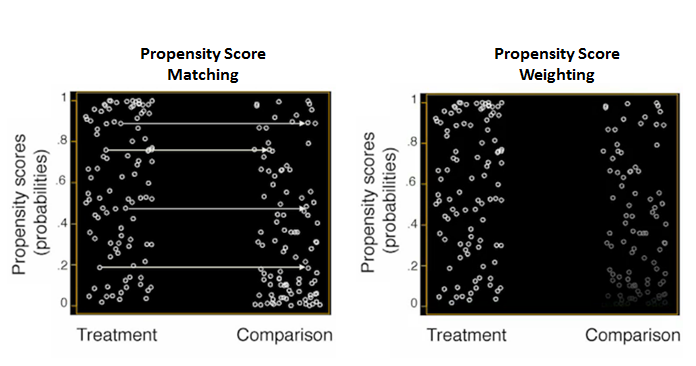
\includegraphics[width=0.8\textwidth]{ps_examples2.png}
    \caption{Taken from TWANG short course \cite{Rand2015}}
\label{fig:psexamp}

\end{figure}
\note{Give a thorough explanation of this}
\end{itemize}


\end{frame}

%ps issues was here
\begin{frame}{IPTW}
\begin{itemize}
\item IPTW: Inverse Probability of Treatment Weights
\item Idea: Weight sample by propensity score so that we get a sample where there is no confounding
\item Weights: $1/e(X)$ for treatment, $1/(1-e(X))$ for control
\item Can be shown that 
\begin{itemize}
 \item $E[\frac{TY(1)}{e(X)}|T=1]=E[Y(1)]$
 \item $E[\frac{(1-T)Y(0)}{1-e(X)}|T=0]=E[Y(0)]$
\end{itemize}
 
\end{itemize}

\note{Justification:
$E[ZY/e(x)]=E[ZY_1/e(x)]=E[E[ZY_1/e(X)]|Y_1,X]$
$=E[Y_1/e(x)E[Z|Y_1,X]]=E[Y_1/e(x) E[Z|X]]$
$=E[Y_1/e(x)e(x)]=E[Y_1]$
}
\end{frame}

\begin{frame}{Propensity Score in MI Setting}
  Mitra and Reiter propose two methods \cite{Mitra2012}
 \begin{itemize}
 
 \item \textit{Within}: Work with propensity score on each of the $m$ MI datasets
 \item \textit{Across}: Average propensity scores across the $m$ datasets and then analyze with the averaged propensities 
  \item Which to use: Dependent on the data

 \end{itemize}

\note{Another method: sample row from each of m datasets to get one sample}
\end{frame}

\section{Propensity Score Application}
\begin{frame}{Propensity Score: Questions To Ask}
\begin{itemize}
\item Generating the propensity score: Generalized Boosted Model- GBM
\begin{itemize}
\item What confounders to put in propensity score model
  \item Stage, race, IDC, breast cancer surgery, HR/HER2 status,
  breast cancer radiation, first met site, number of prior treatments, ECOG score,
  localized brain mets treatment, age at brain met, type of brain mets, brain met controlled
\end{itemize}
\item What estimand do we care about? ATE
\end{itemize} 
\end{frame}



\begin{frame}{Verifying Balance}
For each IPTW MI dataset...
\begin{itemize}
\item Need the distribution of the groups to be similar
\begin{itemize}
\item Standardized bias: $|\bar{X}_{k1}-\bar{X}_{k0}|/ \hat{\sigma}_k$
\item Kolmogorov-Smirnov (KS) test 
\end{itemize}
\item Need to be sure that propensity scores are between 0 and 1
\end{itemize}
\end{frame}


%add ps histo here
\begin{frame}{Balance Checks}
  \begin{figure}[h!]
  \centering
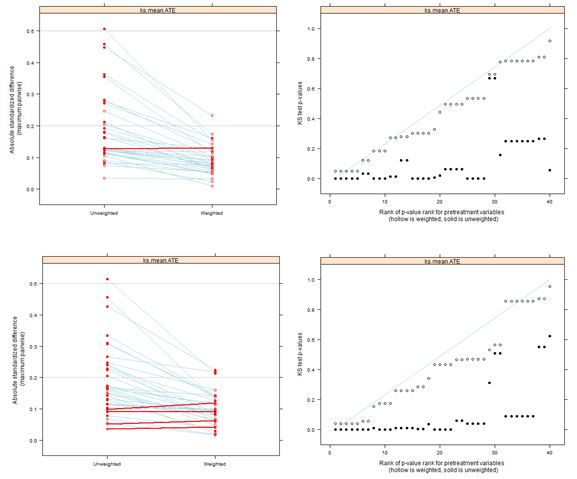
\includegraphics[width=.8\textwidth]{balance_diagnosis} 
  \caption{Selected Balance Diagnostics}
\label{fig:balcheck}
\end{figure}

\end{frame}

\begin{frame}{Results of IPTW: Chemotherapeutic}
 \begin{table}[]
\centering
\adjustbox{max height=\dimexpr\textheight-5.5cm\relax,
           max width=\textwidth}{
\begin{tabular}{|c|c|c|c|c|c|c|c|c|c|c|c|}
\hline
               & \multicolumn{2}{c|}{AC Unweighted} &  & \multicolumn{2}{c|}{AC IPTW} &  & \multicolumn{2}{c|}{MI unweighted} &  & \multicolumn{2}{c|}{MI IPTW} \\ \hline
               & HR           & 95\% CI             &  & HR        & 95\% CI          &  & HR           & 95\% CI             &  & HR         & 95\% CI         \\ \hline
Cape. vs none  & 0.396        & (0.325,0.482)       &  & 0.655     & (0.481,0.894)    &  & 0.484        & (0.400,0.585)       &  & 0.702          & (0.543,0.906)           \\ \hline
Other vs none  & 0.336        & (0.287,0.394)       &  & 0.567     & (0.46,0.754)     &  & 0.413        & (0.354,0.481        &  & 0.593          & (0.470,0.748)           \\ \hline
Cape. vs other & 1.179        & (0.983,1.416)       &  & 1.156     & (0.966,1.383)    &  & 1.173        & (0.981,1.402)       &  & 1.183          & (0.998,1.404)           \\ \hline
\end{tabular}
}
\caption{Chemotherapeutic ATE with IPTW weights, AC and MI}

\end{table}


\begin{table}[]
\centering
\adjustbox{max height=\dimexpr\textheight-5.5cm\relax,
           max width=\textwidth}{
\begin{tabular}{|c|c|c|c|c|c|c|c|c|c|c|c|}
\hline
               & \multicolumn{2}{c|}{AC Unweighted} &  & \multicolumn{2}{c|}{AC IPTW} &  & \multicolumn{2}{c|}{MI unweighted} &  & \multicolumn{2}{c|}{MI IPTW} \\ \hline
               & HR           & 95\% CI             &  & HR        & 95\% CI          &  & HR           & 95\% CI             &  & HR        & 95\% CI          \\ \hline
Cape. vs none  & 0.687        & (0.530,0.891)       &  & 0.603     & (0.443,0.820)    &  & 0.752        & (0.595,0.952)       &  & 0.701     & (0.536,0.917)    \\ \hline
Other vs none  & 0.521        & (0.416,0.653)       &  & 0.452     & (0.340,0.602)    &  & 0.579        & (0.474,0.707)       &  & 0.532     & (0.416,0.681)    \\ \hline
Cape. vs other & 1.318        & (1.078,1.612)       &  & 1.334     & (1.109,1.604)    &  & 1.300        & (1.076,1.570)       &  & 1.317     & (1.100,1.579)    \\ \hline
\end{tabular}
}
\caption{Chemotherapeuic ATE, Doubly Robust, AC, MI}
\label{chemorobust}
\end{table}

\end{frame}

\begin{frame}{Results of IPTW: HER2 Directed}

\begin{table}[]
\centering
\adjustbox{max height=\dimexpr\textheight-5.5cm\relax,
           max width=\textwidth}{
\begin{tabular}{|l|c|c|c|c|c|c|c|c|c|c|c|}
\hline
                   & \multicolumn{2}{c|}{AC Unweighted}                              & \multicolumn{1}{l|}{} & \multicolumn{2}{c|}{AC IPTW}                                    & \multicolumn{1}{l|}{} & \multicolumn{2}{c|}{MI Unweighted}                              & \multicolumn{1}{l|}{} & \multicolumn{2}{c|}{MI IPTW}                                    \\ \hline
                   & HR                         & 95\% CI                            &                       & HR                         & 95\% CI                            &                       & HR                         & 95\% CI                           &                       & HR                         & 95\% CI                            \\ \hline
Lapat. vs none     & 0.467                      & (0.355,0.616)                      &                       & 0.571                      & (0.381,0.855)                      &                       & 0.474                      & (0.362,0.622)                     &                       & 0.485                      & (0.304,0.775)                      \\ \hline
Trastuz. vs none   & 0.488                      & (0.398,0.597)                      &                       & 0.566                      & (0.421,0.759)                      &                       & 0.506                      & (0.417,0.614)                     &                       & 0.480                      & (0.313,0.735)                      \\ \hline
Lapat. vs Trastuz. & \multicolumn{1}{l|}{0.958} & \multicolumn{1}{l|}{(0.693,1.324)} & \multicolumn{1}{l|}{} & \multicolumn{1}{l|}{1.009} & \multicolumn{1}{l|}{(0.680,1.496)} & \multicolumn{1}{l|}{} & \multicolumn{1}{l|}{0.927} & \multicolumn{1}{l|}{(0.673,1.28)} & \multicolumn{1}{l|}{} & \multicolumn{1}{l|}{1.011} & \multicolumn{1}{l|}{(0.763,1.338)} \\ \hline
\end{tabular}
}
\caption{HER2 directed ATE with IPTW weights, AC and MI}
\label{tab:lapatonly}
\end{table}

\begin{table}[]
\centering
\adjustbox{max height=\dimexpr\textheight-5.5cm\relax,
           max width=\textwidth}{
\begin{tabular}{|c|c|c|c|c|c|c|c|c|c|c|c|}
\hline
                   & \multicolumn{2}{c|}{AC Unweighted} &  & \multicolumn{2}{c|}{AC IPTW} &  & \multicolumn{2}{c|}{MI Unweighted} &  & \multicolumn{2}{c|}{MI IPTW} \\ \hline
                   & HR          & 95\% CI              &  & HR        & 95\% CI          &  & HR           & 95\% CI             &  & HR         & 95\% CI            \\ \hline
Lapat. vs none     & 0.468       & (0.316,0.692)        &  & 0.514     & (0.331,0.798)    &  & 0.524        & (0.367,0.747)       &  & 0.410      & (0.257,0.652)      \\ \hline
Trastuz. vs none   & 0.447       & (0.328,0.6089)       &  & 0.456     & (0.328,0.632)    &  & 0.511        & (0.381,0.685)       &  & 0.388      & (0.249,0.602)      \\ \hline
Lapat. vs Trastuz. & 1.048       & (0.704,1.560)        &  & 1.128     & (0.726,1.754)    &  & 1.026        & (0.713,1.477)       &  & 1.057      & (0.788,1.417)      \\ \hline
\end{tabular}
}
\caption{HER2 directed ATE with IPTW weights, double robust}
\label{lapatfull}
\end{table}
 
\end{frame}

